\newcommand{\plotfraction}{0.9}

In this section, we evaluate the performance of different synchronization protocols in dxex.
We also compare to adevs, currently one of the most efficient simulation kernels~\cite{DEVSSurvey}, to show that our modularity does not impede performance.
CPU time and memory usage is compared for both sequential and parallel simulation.

We start off with a comparison of sequential simulation, to show how adevs and dxex relate in this simple case.
For the parallel simulation benchmarks, results are presented for both conservative and optimistic synchronization.

For all benchmarks, results are well within a 5\% deviation of the average, such that only the average is used in the remainder of this section.
The same compilation flags were used for both adevs and dxex benchmarks (``\texttt{-O3 -flto}'').
To guarantee comparable results, no I/O was performed during benchmarks.
Before benchmarking, simulation traces were used to verify that adevs and dxex return exactly the same simulation results.
Benchmarks were performed using Linux, but our simulation tool works equally well on Windows and Mac.
The exact parameters for each benchmark can be found in the repository, as well as the data used in this paper. 

\subsection{Benchmarks}
We use three different benchmarks, which cover different aspects of the simulation kernel:
\begin{enumerate}
    \item The \textit{Queue} model, based on the \textit{HI} model of DEVStone~\cite{DEVStone}, creates a chain of hierarchically nested atomic \textsf{DEVS} models.
          A single generator pushes events into the queue, which are processed by the processors after a random delay.
          It takes two parameters: width and depth, which determine the width and depth of the hierarchy.
          This benchmark shows how the complexity of the simulation kernel behaves for an increasing amount of atomic models, and an increasingly deep hierarchy.
          An example for width and depth 2 is shown in Figure~\ref{fig:queue_model}.

    \item The \textit{PHOLD} model, presented by~\cite{PHOLD}, creates $n$ atomic models, where each model has exactly $n-1$ output ports.
          Each atomic model is directly connected to every other atomic model.
          After a random delay, an atomic model sends out an event to a randomly selected output port.
          Output port selection happens in two phases: first it is decided whether the event should be sent to an atomic model at the same node.
          Afterwards, a uniform selection is made between the remaining ports.
          The model takes one parameter: the percentage of remote events, which determines the fraction of messages routed to other nodes.
          This benchmark shows how the simulation kernel behaves in the presence of many local or remote events.
          An example for four models, split over two nodes, is shown in Figure~\ref{fig:PHOLD_model}.

    \item The \textit{HighInterconnect} model, a merge of PHOLD~\cite{PHOLD} and the \textit{HI} model of DEVStone~\cite{DEVStone}, creates $n$ atomic models, where each model has exactly one output port.
          Similar to PHOLD, all models are connected to one another, but all through the same port: every model receives each generated event.
          The model takes one parameter: the number of models.
          This benchmark investigates the complexity of event routing, and how the simulation kernel handles many simultaneous events.
          An example for four models is shown in Figure~\ref{fig:interconnect_model}.
\end{enumerate}

\newcommand{\modelfraction}{0.65}

\begin{figure}
    \center
    \includegraphics[width=\columnwidth]{fig/queue_model.pdf}
    \caption{Queue model for depth and width 2.}
    \label{fig:queue_model}

    \includegraphics[width=\modelfraction\columnwidth]{fig/interconnect_model.pdf}
    \caption{HighInterconnect model for three models.}
    \label{fig:interconnect_model}

    \includegraphics[width=\modelfraction\columnwidth]{fig/phold_model.pdf}
    \caption{PHOLD model for three models.}
    \label{fig:PHOLD_model}
\end{figure}

\subsection{Sequential Simulation Execution Time}
Despite our core contribution being on parallel simulation, we still value a comparison of sequential simulation results.
First, and foremost, parallel simulation results are tightly linked to sequential simulation results.
Parallel simulation is achieved through synchronization of multiple sequential simulation kernels.
Second, parallel simulation results are validated through the use of adevs.
To provide a well-founded comparison to adevs in the parallel simulation benchmarks, sequential simulation results also need to be compared.

Only the Queue and HighInterconnect models are relevant for sequential simulation, so we do not use the PHold model yet.

\subsubsection{Queue}
In the Queue model, we increase both width and depth simultaneously.
For example, the $400$ models configuration is obtained with a width and depth of $20$.
As can be seen in Figure~\ref{fig:Queue_benchmark}, dxex considerably outperforms adevs.
Through profiling, we found that adevs spends much time routing the simulation messages (\textit{e.g.}, \textit{*} and \textit{@} messages, defined by the abstract simulator~\cite{AbstractSimulator}) through the hierarchy, whereas dxex avoids this through its flattened model structure.
Both simulation tools have similar complexities, though dxex is much faster thanks to its more efficient simulation control algorithms.

\begin{figure}
    \center
	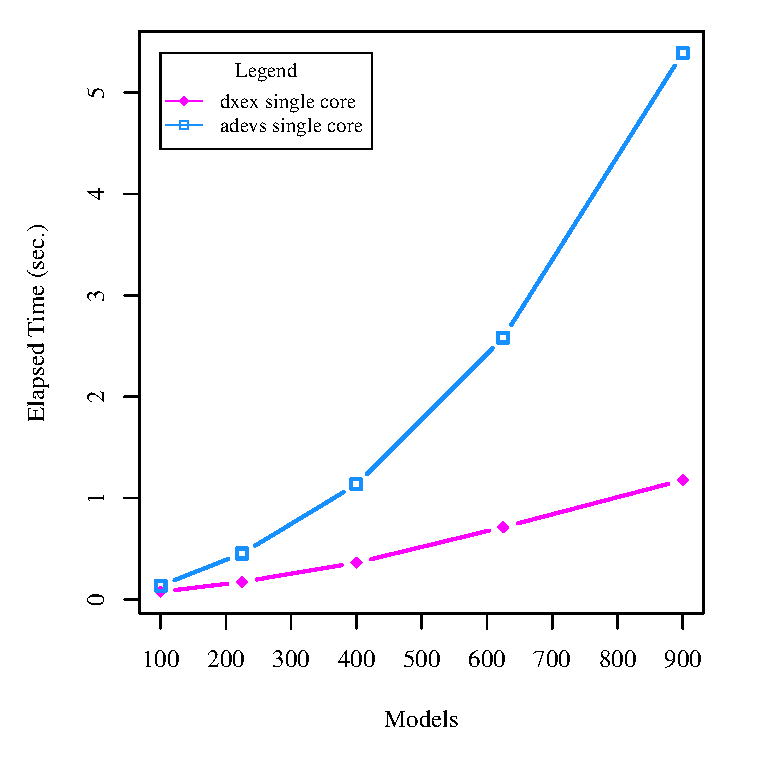
\includegraphics[width=\plotfraction\columnwidth]{fig/queue_sequential.eps}
	\caption{Queue benchmark results for sequential simulation.}
	\label{fig:Queue_benchmark}
\end{figure}

\subsubsection{HighInterconnect}
In the HighInterconnect model, we increase the number of atomic models, thus quadratically increasing the number of couplings and the number of external transitions.
As can be seen in Figure~\ref{fig:Interconnect_benchmark}, adevs outperforms dxex by a fair margin.
Analysis showed that this is caused by the high amount of exchanged events: event creation is much slower in dxex than it is in adevs, despite dxex's use of memory pools.

\begin{figure}
    \center
	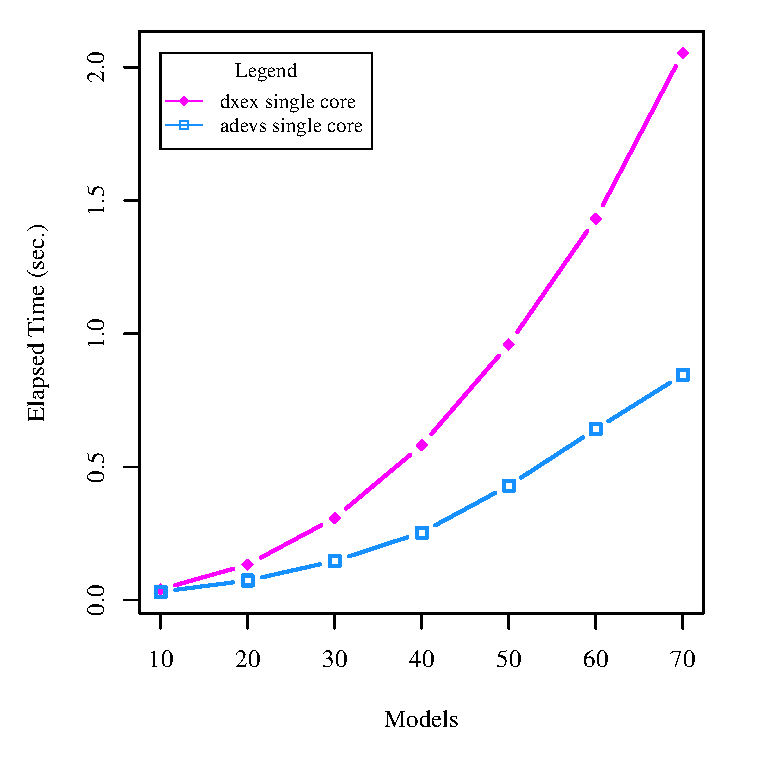
\includegraphics[width=\plotfraction\columnwidth]{fig/interconnect_sequential.eps}
	\caption{Interconnect benchmark results for sequential simulation.}
	\label{fig:Interconnect_benchmark}
\end{figure}

\subsection{Parallel Simulation Execution Time}
Next we analyse parallel simulation of our previously defined benchmarks.
For dxex, we mention results of both conservative and optimistic synchronization.
Since adevs supports only conservative synchronization, we don't mention optimistic synchronization results there.
All experiments were performed using up to six simulation nodes, executed on a hexa-core machine.

We highlight two main results:
(1) dxex conservative synchronization is competitive with adevs;
(2) dxex optimistic synchronization is sometimes more efficient than conservative synchronization.
This shows that our contribution, offering both conservative and optimistic synchronization, is indeed beneficial for a general-purpose simulation tools.

\subsubsection{Queue}
In the Queue model, we allocate the chain of models such that each node is responsible for a series of connected models.
This minimizes the number of inter-node messages.
As the model is a queue, however, models further in the chain only activate later in the simulation.
Since these are allocated to separate nodes, some nodes remain idle until simulation has progressed sufficiently far.

Similar to the sequential benchmarks, Figure~\ref{fig:queue_benchmark_parallel} shows that dxex outperforms adevs, but now in terms of speedup.
Results indicate that our implementation of conservative synchronization achieves much higher speedups than adevs.
Approaching near linear speedup, this simulation is the ideal case for our conservative implementation, as there are no dependency cycles between models.
Conservative synchronization also seems to be better than optimistic synchronization in this case, at the cost of providing the lookahead.

\begin{figure}
    \center
	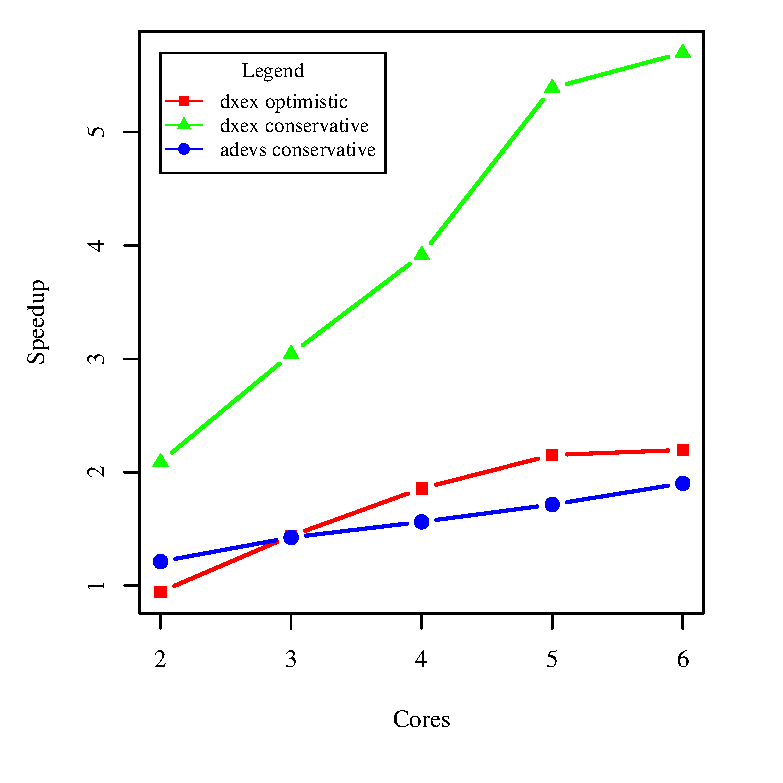
\includegraphics[width=\plotfraction\columnwidth]{fig/queue_parallel.eps}
	\caption{Queue benchmark results for parallel simulation of a model of fixed size.}
	\label{fig:queue_benchmark_parallel}
\end{figure}

\subsubsection{PHold}
In the Phold model, we first investigate the influence of the fraction of remote events on the speedup.
When remote events are rare, optimistic synchronization rarely has to roll back, thus increasing performance.
With more common remote events, however, optimistic synchronization quickly slows down due to frequent rollbacks.
Conservative synchronization, on the other hand, is mostly unconcerned with the number of remote events: the mere fact that a remote event can happen, causes it to block.
Even though a single synchronization protocol is always ideal in this case, it already shows that different synchronization protocols respond differently to a changing model.
Adevs is again significantly slower during conservative synchronization.
Analysis of profiling results shows that exception handling in adevs is the main cause. 
To keep the models equivalent, the adevs version does not provide the \{begin,end\}Lookahead methods, which accounts for the exception handling.

\begin{figure}
    \center
    \includegraphics[width=\plotfraction\columnwidth]{fig/phold_speedup_remotes.eps}
    \caption{Phold benchmark results for parallel simulation using six cores, 4 atomics per node, with varying fraction of remote events.}
\end{figure}

We further verify that our contribution fulfills our projected use case: a single model that can be tweaked to favor either conservative or optimistic synchronization.
We slightly modified the Phold benchmark, to include high-priority events.
Contrary to normal events, high-priority events happen almost instantaneously, restricting lookahead to a very small value.
Even when normal events occur most often, conservative synchronization always blocks until it can make guarantees.
Optimistic synchronization, however, simply goes forward in simulation time and rolls back when these high-priority events happen.
This situation closely mimics the case made in the comparison between both synchronization algorithms by~\cite{FujimotoBook}.

Figure~\ref{fig:phold_priority} shows how simulation performance is influenced by the fraction of these high-priority events.
If barely any high-priority events occur, conservative synchronization is penalized due to its excessive blocking, which often turned out to be unnecessary.
When many high-priority events occur, optimistic synchronization is penalized due to its mindless progression of simulation, which frequently needs to be rolled back.
Results show that there is no single perfect synchronization algorithm for this model: depending on configuration, either synchronization protocol might be better.
We have shown that our contribution is invaluable for high performance simulation: depending on the expected behaviour, modellers can choose the most appropriate synchronization protocol.

\begin{figure}
    \center
    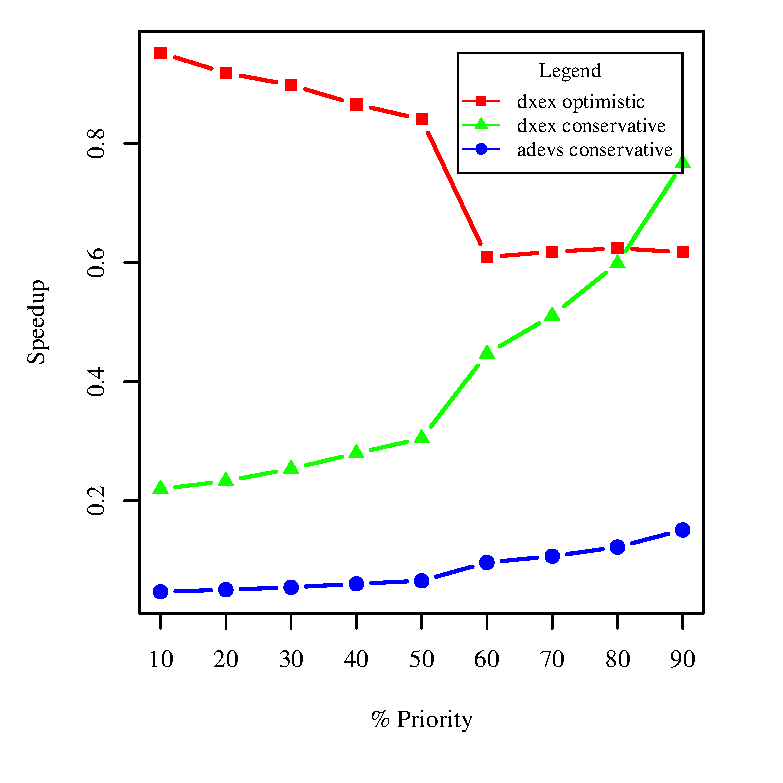
\includegraphics[width=\plotfraction\columnwidth]{fig/phold_speedup_priority.eps}
    \caption{Phold benchmark results for parallel simulation using six cores, with varying amount of high-priority events.}
    \label{fig:phold_priority}
\end{figure}

\subsubsection{Interconnect}
In the Interconnect model, we determine how broadcast communication is supported across multiple nodes.
The number of models is now kept constant at eight.
Results are shown in Figure~\ref{fig:interconnect_benchmark_parallel}.
When the number of nodes increases, performance decreases due to increasing contention in conservative simulation and an increasing number of of rollbacks in optimistic simulation.
All models depend on each other and have no computational load whatsoever, negating any possible performance gain by executing the simulation in parallel.

\begin{figure}
    \center
    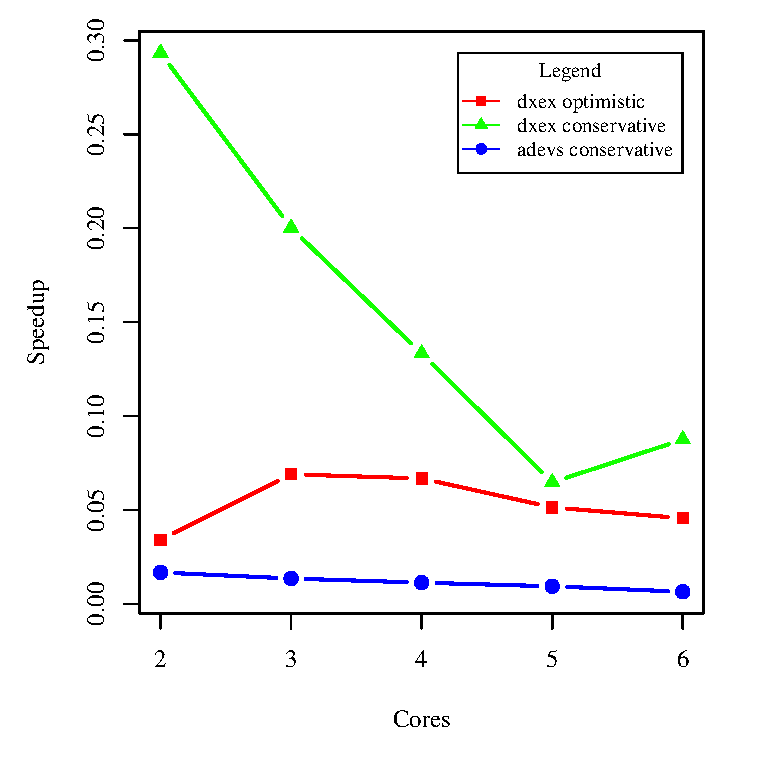
\includegraphics[width=\plotfraction\columnwidth]{fig/interconnect_parallel.eps}
    \caption{Interconnect benchmark results for parallel simulation.}
    \label{fig:interconnect_benchmark_parallel}
\end{figure}

\subsection{Memory Usage}
Apart from simulation execution time, memory usage during simulation is also of great importance.
While execution time only becomes a problem if it takes way too long, coming short only a bit of memory can make simulation unfeasible.
We therefore also investigate memory usage of different synchronization protocols, and again compare to adevs.

We do not tackle the problem of states that become too large for a single machine to hold.
This problem can be mitigated by distribution over multiple machines, which neither dxex or adevs support.

\subsubsection{Remarks}
Both dxex and adevs use \texttt{tcmalloc} as memory allocator, allowing for thread-local allocation.
Additionally, dxex uses memory pools to further reduce the frequency of expensive system calls (\textit{e.g.}, malloc and free).
\texttt{tcmalloc} only gradually releases memory back to the OS, whereas our pools will not do so at all.
Due to our motivation for memory usage analysis, we will only measure peak allocation.
Profiling is done using Valgrind's massif tool~\cite{Nethercote:2007:VFH:1273442.1250746}.

\subsubsection{Results}
Figure~\ref{fig:memory} shows the memory used by the different benchmarks.
Results are in megabytes, and show the total memory footprint of the running application (\textit{i.e.}, text, stack, and heap).

Unsurprisingly, optimistic synchronization results show very high memory usage due to the saved states.
Note the logarithmic scale that was used for this reason.
Optimistic synchronization results vary heavily depending on thread scheduling by the operating system, as this influences the drift between nodes.
Comparing similar approaches, we notice that dxex and adevs have very similar memory use.

Conservative simulation always uses more memory than sequential simulation, as is to be expected.
Additional memory is required for the multiple threads, but also to store all events that are processed simultaneously.

For the Phold benchmark, adevs using conservative synchronization took too long using our profiling tool, and was therefore aborted.
Therefore, no results are shown for adevs.

\begin{figure}
    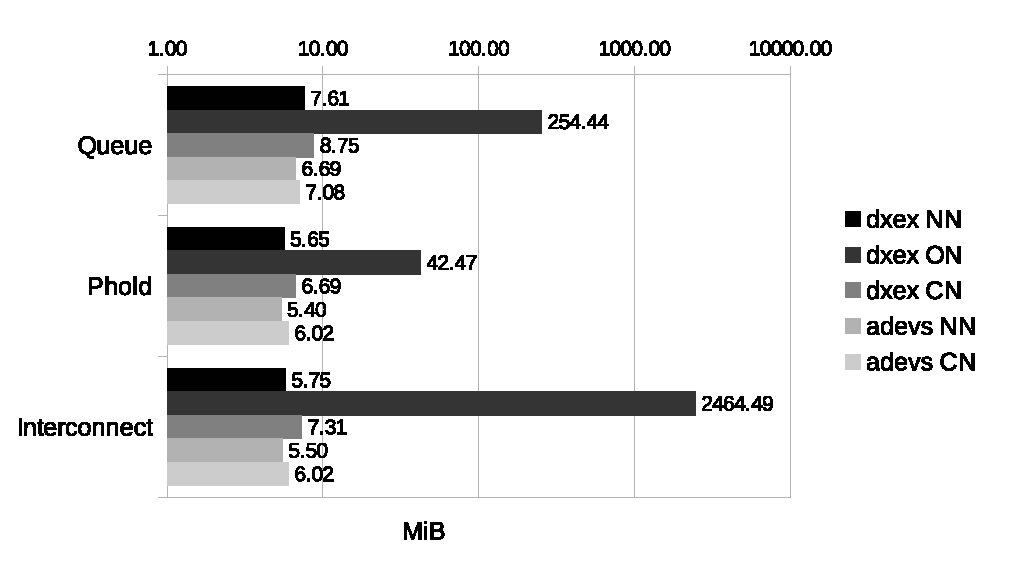
\includegraphics[width=\columnwidth]{fig/memory_voorlopig.eps}
    \caption{Memory usage results.}
    \label{fig:memory}
\end{figure}
